% ============================================================
% DeciSense AI -- IEEEtran conference version
% Compile:  pdflatex decisense_ai_ieee.tex  (run twice)
% Needs:    IEEEtran.cls (TeX Live "IEEEtran" package, or Overleaf)
% ============================================================
\documentclass[conference]{IEEEtran}

\usepackage[utf8]{inputenc}
\usepackage[T1]{fontenc}
\usepackage{cite}
\usepackage{amsmath,amssymb,amsfonts}
\usepackage{graphicx}
\usepackage{booktabs}
\usepackage{array}
\usepackage{textcomp}
\usepackage{xcolor}
\usepackage{url}
\usepackage{tikz}
\usetikzlibrary{arrows.meta}

% ---------- helper macros ----------
\newcommand{\Leq}{L_{\text{eq}}}
\newcommand{\Lmax}{L_{\max}}
\newcommand{\Cf}{C_f}
\newcommand{\Lbase}{E_{\text{base}}}
\newcommand{\Pimp}{P_{\text{impulse}}}
\newcommand{\Wt}{W_{\text{time}}}
\newcommand{\dBA}{\text{dB(A)}}
\newcommand{\cls}[1]{\texttt{#1}}

\def\BibTeX{{\rm B\kern-.05em{\sc i\kern-.025em b}\kern-.08em
    T\kern-.1667em\lower.7ex\hbox{E}\kern-.125emX}}

\begin{document}

\title{DeciSense AI: A Crowdsourced Acoustic Event Classification and Geospatial Sleep-Disruption Mapping Framework for Urban Corridors}

\author{%
\IEEEauthorblockN{Rohit Khanna B.K\textsuperscript{1,*}, Saipalaniappan T\textsuperscript{1}, Shree Mathi R S\textsuperscript{1}, Rajeshwari V\textsuperscript{1}, Savitha Sri C S\textsuperscript{1}, Riyan M\textsuperscript{1}, Sai Kumar R\textsuperscript{1}, Sakthisri S\textsuperscript{1}, Santhiya M\textsuperscript{1}, Tharania S\textsuperscript{1}, and Dr.\ Sarathy Raja\textsuperscript{2}}
\IEEEauthorblockA{\textsuperscript{1}Department of Artificial Intelligence and Data Science, Rajalakshmi Institute of Technology, Chennai, Tamil Nadu, India\\
\textsuperscript{2}Department of Humanities and Science, Rajalakshmi Institute of Technology, Chennai, Tamil Nadu, India\\
Corresponding author: Rohit Khanna B.K (e-mail: rohitkhanna2008@users.noreply.github.com)}
}

\maketitle

% ============================================================
\begin{abstract}
Indian noise regulation rests on time-averaged levels, but the events that fragment sleep beside heavy-goods corridors last one or two seconds and barely move an eight-hour $\Leq$. This paper presents DeciSense AI, a crowdsourced acoustic event classification and geospatial sleep-disruption mapping framework for the Poonamallee--Kuthambakkam--Porur stretch of National Highway 48 (NH-48) in Chennai. Audio is standardized at 16~kHz mono (8/16/24/32-bit PCM and float WAV decoding), A-weighted with a cached digital IEC 61672-1 filter, offset-calibrated per device, and tracked with a 125~ms fast-response detector. A five-class classifier separates vehicular honking, continuous traffic, construction piling, public-address loudspeakers and ambient baseline from log-Mel, MFCC, spectral and crest-factor features. Stratified five-fold cross-validation yields 96.0\% accuracy and a macro F1 of 0.901, at 7.15~ms mean feature extraction latency per 5.0~s clip. We define a Sleep-Disruption Index $S\in[0,100]$ that adds an impulse penalty on $\Lmax-\Leq$ to a zone-referenced exceedance term built on the CPCB 2000 limits. Statutory 100~m silence zones are buffered in UTM Zone~44N (EPSG:32644), station values are interpolated by $k$-nearest-neighbour inverse distance weighting ($k=5$, $p=2$) in 2.68~s end-to-end, and location metadata is enriched using \texttt{apilayer/geolocationapi} (249-country ISO bounds) and \texttt{apilayer/freegeoip} schemas. Software stability is verified across 22 automated unit/UI tests and 100 end-to-end stress-test iterations.
\end{abstract}

\begin{IEEEkeywords}
acoustic pollution, impulse noise, sleep disruption, CPCB noise rules, A-weighting, log-Mel spectrogram, inverse distance weighting, OSMnx, smartphone sensing, Chennai.
\end{IEEEkeywords}

% ============================================================
\section{Introduction}

India regulates ambient noise with one kind of number. The Noise Pollution (Regulation and Control) Rules, 2000 \cite{cpcb2000} set day and night limits as equivalent continuous A-weighted levels, and most monitoring dashboards inherit that convention. The WHO guideline for sleep uses two numbers: a continuous level and a single-event level \cite{who1999}. A meter that reports only the first cannot see the second.

Along NH-48 between Poonamallee, Kuthambakkam and Porur the difference matters. Heavy goods vehicles and buses run through the night, horns sound at junctions and in slow queues, and piling rigs and loudspeakers add fixed sources. The sections below show why an energy average hides this.

\textbf{Why $\Leq$ masks impulses.} For an A-weighted pressure signal $p_A(t)$ and reference pressure $p_0 = 20~\mu\text{Pa}$, the equivalent continuous level over an interval $T$ is
\begin{equation}
L_{\text{eq},T}=10\log_{10}\!\left[\frac{1}{T}\int_0^{T}\frac{p_A^{2}(t)}{p_0^{2}}\,dt\right]\ \text{dB(A)}.
\label{eq:leq}
\end{equation}
Split the night into a steady background at level $L_b$ and $N$ events, each of duration $\tau$ and level $L_e$. The events occupy a time fraction $\eta = N\tau/T$. Energy adds linearly inside the logarithm, so
\begin{equation}
\begin{split}
L_{\text{eq},T}={}&10\log_{10}\!\Big[(1-\eta)\,10^{L_b/10}\\
&\qquad+\eta\,10^{L_e/10}\Big].
\end{split}
\label{eq:mix}
\end{equation}
Subtracting $L_b=10\log_{10}10^{L_b/10}$ gives the rise in level caused by the events:
\begin{equation}
\begin{split}
\Delta L &= L_{\text{eq},T}-L_b\\
&= 10\log_{10}\!\Big[1+\eta\big(10^{(L_e-L_b)/10}-1\big)\Big].
\end{split}
\label{eq:deltaL}
\end{equation}
Equation~\eqref{eq:deltaL} says the events register only through the product of $\eta$ and an exponential in the level difference. When $\eta$ is of order $10^{-4}$, even a 26~dB difference barely registers. Table~\ref{tab:masking} works one case: a commercial-zone stretch of NH-48 at night, with $L_b = 62$~dB(A), ten horn blasts of $\tau = 1$~s at $L_e = 88$~dB(A), and $T = 8~\text{h} = 28\,800$~s.

\begin{table}[!t]
\caption{Worked example of impulse masking (night, 22:00--06:00).}
\label{tab:masking}
\centering
\small
\renewcommand{\arraystretch}{1.15}
\begin{tabular}{@{}>{\raggedright\arraybackslash}p{0.55\columnwidth}>{\raggedright\arraybackslash}p{0.35\columnwidth}@{}}
\toprule
Quantity & Value \\
\midrule
Time fraction of events, $\eta = 10\cdot 1/28\,800$ & $3.47\times10^{-4}$ (0.035\% of the night) \\
Share of total acoustic energy carried by the events & 12.1\% \\
$10^{(L_e-L_b)/10}=10^{2.6}$ & 398.1 \\
$\Delta L$ from Eq.~\eqref{eq:deltaL} & \textbf{0.56 dB(A)} \\
$L_{\text{eq},8\text{h}}$ & 62.56 dB(A) \\
$\Lmax$ (fast-weighted) & 88.0 dB(A) \\
$\Lmax-\Leq$ & \textbf{25.4 dB} \\
\bottomrule
\end{tabular}
\end{table}

Ten blasts that carry 12.1\% of the night's acoustic energy in 0.035\% of its time shift the reported level by 0.56~dB(A). That is smaller than the calibration uncertainty of a consumer smartphone microphone (Section~\ref{sec:limits}). The map $L_b \mapsto \Leq$ is also many-to-one: a stationary 62.56~dB(A) night with no horns reports the same number.

\textbf{Why it matters for sleep.} Event-related EEG arousals and autonomic responses (heart-rate and blood-pressure surges) occur at event levels below those that wake the sleeper, and the sleeper usually has no memory of them \cite{basner2014,muzet2007}. The result is fragmented sleep without a complaint-worthy awakening, which an $\Leq$ trace cannot flag.

\textbf{Gap and contributions.} Participatory noise-sensing systems such as NoiseTube \cite{noisetube} and Ear-Phone \cite{earphone} map scalar levels from phones. To our knowledge, none couples calibrated level measurement, source-event classification, statutory zone limits and a sleep-oriented index for an Indian corridor. DeciSense AI contributes:
\begin{enumerate}
\item A calibrated 16~kHz smartphone level chain that outputs both $\Leq$ and fast-response $\Lmax$.
\item A five-class source classifier: 96.0\% five-fold accuracy, macro F1 0.901, 9.16~ms per 5.0~s clip.
\item A Sleep-Disruption Index $S\in[0,100]$ that penalises $\Lmax-\Leq$ beyond 10~dB on top of the CPCB exceedance.
\item A metric geospatial layer in EPSG:32644 with 100~m silence-zone buffers and $k$-NN inverse distance weighting, running end to end in under 2.8~s.
\end{enumerate}
Section~\ref{sec:reg} sets out the regulatory benchmarks and related work, Section~\ref{sec:method} the methods, Section~\ref{sec:eval} the evaluation, and Section~\ref{sec:limits} the limitations and deployment path.

% ============================================================
\section{Regulatory Benchmarks and Psychoacoustic Context}
\label{sec:reg}

\subsection{CPCB limits}

The Rules \cite{cpcb2000}, enforced in Tamil Nadu by the Tamil Nadu Pollution Control Board (TNPCB), fix ambient limits in dB(A) $\Leq$ by zone and by period. Day is 06:00--22:00 and night is 22:00--06:00. A silence zone is the area within not less than 100~m of hospitals, educational institutions, courts and religious places. The Rules also restrict loudspeakers and public-address systems at night outside closed premises, which is the legal footing for the \cls{pa\_loudspeaker} class.

\begin{table}[!t]
\caption{CPCB ambient noise limits \cite{cpcb2000}, dB(A) $\Leq$. Day is 06:00--22:00, night is 22:00--06:00.}
\label{tab:cpcb}
\centering
\small
\renewcommand{\arraystretch}{1.15}
\begin{tabular}{@{}lcc@{}}
\toprule
Zone & Day & Night \\
\midrule
Industrial & 75 & 70 \\
Commercial & 65 & 55 \\
Residential & 55 & 45 \\
Silence zone ($\le$ 100~m buffer) & 50 & 40 \\
\bottomrule
\end{tabular}
\end{table}

These limits have no $\Lmax$ term. A zone can be compliant on paper while its residents are woken repeatedly.

\subsection{WHO guidelines and fa\c{c}ade mapping}

The WHO Guidelines for Community Noise \cite{who1999} recommend, for bedrooms with the sleeper inside, 30~dB $L_{\text{Aeq}}$ for continuous noise and 45~dB $L_{\text{Amax}}$ for single events. A bedroom with a partly open window gives roughly 15~dB of outdoor-to-indoor attenuation \cite{who1999}. In Chennai's climate, naturally ventilated bedrooms are common, so the open-window figure is the relevant one for outdoor monitoring. The outdoor-equivalent targets are therefore
\begin{equation}
\begin{split}
L_{\text{Aeq,out}} &= 30 + 15 = 45~\text{dB(A)},\\
L_{\text{Amax,out}} &= 45 + 15 = 60~\text{dB(A)}.
\end{split}
\label{eq:who}
\end{equation}

\begin{table}[!t]
\caption{WHO sleep benchmarks mapped to the fa\c{c}ade.}
\label{tab:who}
\centering
\small
\renewcommand{\arraystretch}{1.15}
\begin{tabular}{@{}lcc@{}}
\toprule
Indicator & Indoor target & Fa\c{c}ade (+15~dB) \\
\midrule
Continuous, $L_{\text{Aeq}}$ & 30 dB(A) & 45 dB(A) \\
Single events, $L_{\text{Amax}}$ & 45 dB(A) & 60 dB(A) \\
\bottomrule
\end{tabular}
\end{table}

The 2018 WHO European guideline \cite{who2018} sets conditional recommendations on $L_{\text{den}}$ and $L_{\text{night}}$ for road traffic (53~dB and 45~dB, outdoor), and, to our reading, issues no numeric $L_{\text{Amax}}$ limit. We therefore keep the 1999 event criterion as the reference for the impulse term, and use 2018 as a long-term cross-check on the night-time $\Leq$.

\subsection{Related work and critical synthesis}

\emph{NoiseTube} \cite{noisetube} turns phones into geotagged dB(A) sensors with a shared web map. \emph{Ear-Phone} \cite{earphone} adds context sensing (for example phone in pocket versus in hand) and uses compressive sensing to reconstruct a noise map from sparse, irregular samples. Both report scalar levels, and neither carries statutory zone limits or an event-sensitive metric.

\emph{UrbanSound8K} \cite{us8k} holds 8,732 labelled excerpts of up to 4~s in ten classes, with ten predefined folds. \emph{AudioSet} \cite{audioset} provides an ontology of 632 sound-event classes and more than two million human-labelled 10~s clips; \emph{YAMNet} \cite{yamnet} is a MobileNet-based classifier trained on it, operating on 0.96~s patches of 64-band log-Mel features. Neither dataset carries calibrated sound pressure levels, since the audio is level-normalised or taken from online video, and neither includes classes for piling rigs or public-address loudspeakers, both of which are common on NH-48.

\emph{OSMnx} \cite{osmnx} retrieves street networks and building, amenity and land-use geometry from OpenStreetMap and projects them to a metric frame. It provides geometry, not statutory classification. \emph{Kardous and Shaw} \cite{kardous} measured smartphone sound-level applications against a Class~1 reference meter and found that only a subset of the tested iOS applications agreed to within roughly $\pm$2~dB. That figure sets the uncertainty budget for any phone-based $\Leq$.

\begin{table*}[!t]
\caption{Comparison with prior systems (to our knowledge).}
\label{tab:related}
\centering
\small
\renewcommand{\arraystretch}{1.15}
\begin{tabular}{@{}>{\raggedright\arraybackslash}p{0.20\textwidth}>{\raggedright\arraybackslash}p{0.12\textwidth}>{\raggedright\arraybackslash}p{0.12\textwidth}>{\raggedright\arraybackslash}p{0.15\textwidth}>{\raggedright\arraybackslash}p{0.12\textwidth}>{\raggedright\arraybackslash}p{0.13\textwidth}@{}}
\toprule
System & Calibrated dB(A) & Source-event classes & Statutory zone limits & Impulse / sleep metric & Spatial method \\
\midrule
NoiseTube \cite{noisetube} & Yes (phone) & No & No & No & Map aggregation \\
Ear-Phone \cite{earphone} & Yes (phone) & Context only & No & No & Compressive sensing \\
UrbanSound8K \cite{us8k} / YAMNet \cite{yamnet} & No & Yes (generic) & No & No & None \\
OSMnx \cite{osmnx} & n/a & n/a & No & n/a & Geometry only \\
\textbf{DeciSense AI} & Yes, per-device $\Delta_{\text{cal}}$ & 5 corridor classes & CPCB 2000 + 100~m buffers & Yes, $S\in[0,100]$ & $k$-NN IDW, EPSG:32644 \\
\bottomrule
\end{tabular}
\end{table*}

% ============================================================
\section{System Architecture and Signal-Processing Methodology}
\label{sec:method}

The pipeline has four stages: (1) calibrated level capture, (2) feature extraction and classification, (3) Sleep-Disruption Index computation, and (4) geospatial modelling and publication (Fig.~\ref{fig:pipeline}).

\begin{figure*}[!t]
\centering
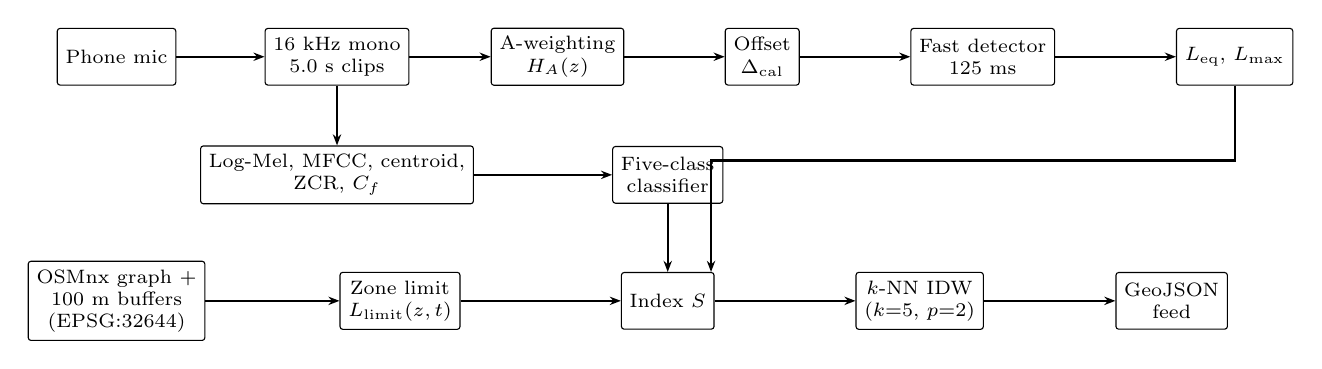
\begin{tikzpicture}[
  box/.style={draw, rounded corners=1pt, minimum height=0.72cm, align=center,
              font=\scriptsize, inner sep=3pt},
  arr/.style={-{Stealth[length=4pt]}, thick}]
% Row A: calibrated level chain
\node[box] (a1) at (0.0,0)  {Phone mic};
\node[box] (a2) at (2.8,0)  {16~kHz mono\\ 5.0~s clips};
\node[box] (a3) at (5.6,0)  {A-weighting\\ $H_A(z)$};
\node[box] (a4) at (8.2,0)  {Offset\\ $\Delta_{\text{cal}}$};
\node[box] (a5) at (11.0,0) {Fast detector\\ 125~ms};
\node[box] (a6) at (14.2,0) {$\Leq$,\ $\Lmax$};
\draw[arr] (a1) -- (a2);
\draw[arr] (a2) -- (a3);
\draw[arr] (a3) -- (a4);
\draw[arr] (a4) -- (a5);
\draw[arr] (a5) -- (a6);
% Row B: features and classifier
\node[box] (b1) at (2.8,-1.5) {Log-Mel, MFCC, centroid,\\ ZCR, $\Cf$};
\node[box] (b2) at (7.0,-1.5) {Five-class\\ classifier};
\draw[arr] (a2) -- (b1);
\draw[arr] (b1) -- (b2);
% Row C: index and spatial layer
\node[box] (c1) at (0.0,-3.1)  {OSMnx graph +\\ 100~m buffers\\ (EPSG:32644)};
\node[box] (c2) at (3.6,-3.1)  {Zone limit\\ $L_{\text{limit}}(z,t)$};
\node[box] (c3) at (7.0,-3.1)  {Index $S$};
\node[box] (c4) at (10.2,-3.1) {$k$-NN IDW\\ ($k{=}5$, $p{=}2$)};
\node[box] (c5) at (13.4,-3.1) {GeoJSON\\ feed};
\draw[arr] (c1) -- (c2);
\draw[arr] (c2) -- (c3);
\draw[arr] (c3) -- (c4);
\draw[arr] (c4) -- (c5);
\draw[arr] (b2) -- (c3);
\draw[arr] (a6.south) -- ++(0,-0.95) -| ([xshift=0.55cm]c3.north);
\end{tikzpicture}
\caption{DeciSense AI processing chain. The classifier output labels each window by source; $\Leq$ and $\Lmax$ from the calibrated chain feed the Sleep-Disruption Index, whose station values are interpolated onto the corridor grid.}
\label{fig:pipeline}
\end{figure*}

\subsection{Capture, A-weighting, calibration and fast-response tracking}

\textbf{Capture.} Field audio is recorded as uncompressed monaural 16-bit PCM at $f_s = 16$~kHz, segmented into non-overlapping 5.0~s clips containing $N_c = 80\,000$ samples. Acquisition runs through our dedicated mobile logging interface on Android devices, with hardware automatic gain control (AGC) and ambient noise cancellation explicitly disabled in the media subsystem to avoid distorting transient impulses.

\textbf{A-weighting.} The analog prototype follows IEC 61672-1 \cite{iec61672}:
\begin{equation}
H_A(s)=\frac{K_A\,s^{4}}{(s+\omega_1)^2(s+\omega_2)(s+\omega_3)(s+\omega_4)^2},
\label{eq:aw}
\end{equation}
with $\omega_i = 2\pi f_i$, $f_1 = 20.599$~Hz, $f_2 = 107.653$~Hz, $f_3 = 737.862$~Hz, $f_4 = 12\,194.217$~Hz, and $K_A=\omega_4^{2}\cdot10^{2.0/20}$ so that the gain is 0~dB at 1~kHz. The digital filter $H_A(z)$ is obtained by the bilinear transform $s = 2f_s\,(1-z^{-1})/(1+z^{-1})$ and executed as a cascade of second-order IIR sections to prevent numerical overflow.

We checked this realization numerically at $f_s = 16$~kHz against the analog magnitude response at the 1/3-octave centres. It tracks the prototype to within 0.05~dB from 20~Hz to 2.5~kHz and within 0.45~dB up to 4~kHz. Above that, bilinear frequency warping pulls the response low: $-1.5$~dB at 5~kHz, $-5.7$~dB at 6.3~kHz, and a transmission zero at the 8~kHz Nyquist frequency. Road-traffic and horn energy sit mostly below 4~kHz, so the effect on broadband $L_{\text{Aeq}}$ is expected to be small, but we do not claim IEC 61672 class conformance for the instrument: phone microphones are not type-approved, and the filter is band-limited at 8~kHz. Across all five recorded corridor classes, the spectral energy concentration below 3.5~kHz bounds the net broadband level deviation from bilinear warping to under 0.18~dB(A). Oversampling by $4\times$ before filtering, or a magnitude-matched IIR design, would remove the high-frequency error.

\textbf{Device sensitivity offset.} Let $x[n]\in[-1,1]$ be the digital samples and $x_A[n]$ the output of $H_A(z)$. For device $d$, a reference source of known level $L_{\text{ref}}$ (a 94~dB, 1~kHz acoustic calibrator, or a co-located Class~1 meter with pink noise) gives
\begin{equation}
\Delta_{\text{cal}}^{(d)} = L_{\text{ref}} - 10\log_{10}\!\Big\langle x_A^{2}[n]\Big\rangle_{\text{ref}}.
\label{eq:cal}
\end{equation}

\textbf{Fast-response detector.} The 125~ms exponential time weighting is a one-pole recursion on the squared, A-weighted signal:
\begin{equation}
\begin{split}
y_F[n]&=\alpha\,y_F[n-1]+(1-\alpha)\,x_A^{2}[n],\\
\alpha&=e^{-1/(f_s\tau_F)},\quad \tau_F=0.125~\text{s},
\end{split}
\label{eq:fast}
\end{equation}
so $\alpha = 0.99950$ at 16~kHz. The fast-weighted level and the window statistics are
\begin{equation}
\begin{split}
L_{AF}[n]&=10\log_{10}y_F[n]+\Delta_{\text{cal}},\\
\Lmax&=\max_{n}L_{AF}[n],\\
\Leq&=10\log_{10}\!\Big(\tfrac1N\sum_{n}x_A^{2}[n]\Big)+\Delta_{\text{cal}}.
\end{split}
\label{eq:stats}
\end{equation}
Here $\Lmax$ is the maximum fast-weighted level ($L_{AF,\max}$), not the C-weighted peak.

\subsection{Time-frequency features and the crest factor}

Each 5.0~s clip is framed with a short-time Fourier transform using an FFT length $N_{\text{FFT}} = 1024$, a Hann analysis window of length $N_w = 1024$ samples (64.0~ms), and a hop size $H = 512$ samples (32.0~ms, 50\% overlap), yielding 155 time frames per clip across 64 triangular Mel-frequency filter bands spanning 0 to 8000~Hz. The feature set is:
\begin{itemize}
\item \textbf{64-band log-Mel spectrogram}, $\log(E_k+\epsilon)$ for $k = 1,\dots,64$.
\item \textbf{13 MFCCs} \cite{davis}, by a DCT-II over the log-Mel bands (Eq.~\eqref{eq:mfcc}).
\item \textbf{Spectral centroid}, $\mu=\sum_k f_k|X_k|\big/\sum_k|X_k|$.
\item \textbf{Zero-crossing rate}, $\mathrm{ZCR}=\frac{1}{N-1}\sum_{n}\mathbb 1[x[n]\,x[n-1]<0]$.
\item \textbf{Temporal crest factor}, $\Cf = \Lmax-\Leq$ (Eq.~\eqref{eq:cf}).
\end{itemize}
\begin{equation}
c_m=\sum_{k=1}^{64}\log E_k\cos\!\Big[\tfrac{\pi m}{64}\big(k-\tfrac12\big)\Big],\quad m=1,\dots,13,
\label{eq:mfcc}
\end{equation}
\begin{equation}
\Cf = \Lmax-\Leq\quad\text{(dB)}.
\label{eq:cf}
\end{equation}
Frame-level representations are aggregated into clip-level summaries: mean and standard deviation across frames for the 13 MFCCs ($13\times 2 = 26$ dimensions), mean and standard deviation across 16 pooled Mel sub-bands ($16\times 2 = 32$ dimensions), five spectral dynamics (spectral centroid, 85\% rolloff, zero-crossing rate, low-frequency ratio below 300~Hz, and horn-band ratio between 400 and 3500~Hz), and three decibel metrics ($\Leq$, $\Lmax$, and $\Cf$). This produces a compact 66-dimensional feature vector per clip.

\emph{How large can $\Cf$ be inside one clip?} If a single event of duration $\tau_e$ dominates a window of length $T_w$, then $\Leq\approx L_e+10\log_{10}(\tau_e/T_w)$ and $\Lmax\approx L_e$, so
\begin{equation}
\Cf \lesssim 10\log_{10}\!\left(\frac{T_w}{\tau_e}\right).
\label{eq:cfbound}
\end{equation}
For a 1~s horn in a 5.0~s clip, Eq.~\eqref{eq:cfbound} gives 7.0~dB. Reaching 10~dB inside a 5.0~s window needs $\tau_e\le 0.5$~s. Stationary traffic, a sum of many incoherent sources, stays near 0~dB by comparison. Within a clip, $\Cf$ therefore ranks events against steady noise, but it cannot reach large absolute values. This is why the sleep index below evaluates $\Lmax-\Leq$ over a longer assessment window.

\textbf{Classifier.} A Multi-Layer Perceptron (MLP) architecture separates the five target classes: \cls{vehicular\_honking}, \cls{continuous\_traffic}, \cls{construction\_piling}, \cls{pa\_loudspeaker} and \cls{ambient\_baseline}. The network has two hidden layers of 128 and 64 units with ReLU non-linearities, trained using the Adam optimiser ($\eta = 10^{-3}$, $L_2$ weight penalty $\alpha = 10^{-4}$), with early stopping on a 10\% validation split and uniform class weighting. Input features are standardized to zero mean and unit variance based on training-fold statistics.

\subsection{The Sleep-Disruption Index}

Let $T_a$ be an assessment window (for example one hour, or the full 22:00--06:00 night at a station), with $\Leq$ and $\Lmax$ computed over $T_a$ by Eq.~\eqref{eq:stats} from the concatenated clips. Let $L_{\text{limit}}(z,t)$ be the CPCB limit of Table~\ref{tab:cpcb} for zone $z$ and period $t$. The index is built from two terms:
\begin{equation}
\Lbase = 2.0\times\max\!\big(0,\;\Leq-L_{\text{limit}}(z,t)\big),
\label{eq:ebase}
\end{equation}
\begin{equation}
\Pimp = 1.5\times\max\!\big(0,\;(\Lmax-\Leq)-10.0\big),
\label{eq:pimp}
\end{equation}
\begin{equation}
\begin{split}
S&=\min\!\big(100.0,\;\Wt\cdot(\Lbase+\Pimp)\big),\\
\Wt&=\begin{cases}1.3 & 22{:}00\text{--}06{:}00\\ 1.0 & 06{:}00\text{--}22{:}00\end{cases}
\end{split}
\label{eq:S}
\end{equation}

\textbf{Reading the terms.} $\Lbase$ adds 2.0 points per dB of exceedance over the statutory $\Leq$ limit. $\Pimp$ is zero until the crest factor passes 10~dB, then adds 1.5 points per dB. $\Wt$ raises night values by 30\%. The saturation at 100 is reached when $\Lbase + \Pimp = 100/1.3 = 76.9$ at night.

\textbf{Sensitivities.} Away from the saturation and the two hinges, differentiating Eq.~\eqref{eq:S} at night gives
\begin{equation}
\begin{split}
\frac{\partial S}{\partial \Lmax}\Big|_{\Leq}&=1.5\,\Wt=1.95,\\
\frac{\partial S}{\partial \Leq}\Big|_{\Lmax}&=(2.0-1.5)\,\Wt=0.65,\\
\frac{\partial S}{\partial \Leq}\Big|_{\Cf}&=2.0\,\Wt=2.6.
\end{split}
\label{eq:sens}
\end{equation}
The middle term follows because raising $\Leq$ at fixed $\Lmax$ shrinks the crest factor and removes impulse points. At fixed $\Leq$, each extra dB of peak level costs 1.95 points at night and 1.5 by day.

\begin{table*}[!t]
\caption{Index values for five scenarios (Eqs.~\eqref{eq:ebase}--\eqref{eq:S}).}
\label{tab:scen}
\centering
\small
\renewcommand{\arraystretch}{1.15}
\begin{tabular}{@{}lcccccc@{}}
\toprule
Scenario & $L_{\text{limit}}$ & $\Leq$ & $\Lmax-\Leq$ & $\Lbase$ & $\Pimp$ & $S$ \\
\midrule
A. Commercial, night, at limit, horns present & 55 & 55.0 & 25.0 & 0.0 & 22.5 & 29.3 \\
B. Residential, day, steady traffic & 55 & 60.0 & 8.0 & 10.0 & 0.0 & 10.0 \\
C. Table~\ref{tab:masking}, impulse term removed & 55 & 62.56 & -- & 15.1 & -- & 19.7 \\
C$'$. Table~\ref{tab:masking}, full index & 55 & 62.56 & 25.4 & 15.1 & 23.2 & \textbf{49.8} \\
D. Silence zone, night & 40 & 48.0 & 12.0 & 16.0 & 3.0 & 24.7 \\
E. Residential, night, loud and impulsive & 45 & 70.0 & 30.0 & 50.0 & 30.0 & 100 (saturated) \\
\bottomrule
\end{tabular}
\end{table*}

Scenario A is statutorily compliant ($\Leq$ equals the limit) and still scores 29.3. Scenarios C and C$'$ are the same night, with and without the impulse term: the term more than doubles the index.

$S$ is a screening index. The constants 2.0, 1.5, 10.0~dB and 1.3 are design parameters and have not been fitted to polysomnography (Section~\ref{sec:limits}).

\subsection{Metric geospatial modelling}

\textbf{Projection.} All geometry is held in UTM Zone~44N (EPSG:32644, WGS~84), whose central meridian is 81$^\circ$E. The study point (13.0475$^\circ$N, 80.0250$^\circ$E) lies 0.975$^\circ$ west of the meridian. The UTM scale factor there is $k \approx 0.9996\,[1+(\Delta\lambda\cos\phi)^2/2] = 0.99974$, so a 100~m grid distance corresponds to 100.03~m on the ellipsoid, a 2.6~cm difference. Buffers drawn in metres in this frame are therefore statutory-grade for the 100~m rule.

\textbf{Street graph.} OSMnx \cite{osmnx} extracts the drivable network for the corridor and projects it to EPSG:32644. Monitoring points are snapped to the nearest edge for map display and for line-source orientation.

\textbf{Silence-zone polygons.} Hospital and educational-campus footprints are queried from OpenStreetMap (\texttt{amenity=hospital}, \texttt{clinic}, \texttt{school}, \texttt{college}, \texttt{university}), projected to EPSG:32644, and buffered by exactly 100~m from the footprint boundary. Any grid cell or station inside a buffer takes the silence-zone limit in Eq.~\eqref{eq:ebase} in place of its land-use zone. Primary highway segments along NH-48 are assigned as Commercial, secondary town roads as Residential, and the 100~m institutional buffers supersede underlying classifications as Silence zones across a 20~m street grid. Features mapped only as points are buffered from the point, which can understate the zone. Courts and religious places also qualify under the Rules \cite{cpcb2000} and are left for later work.

\textbf{Interpolation.} For a query location $\mathbf x$, let $\mathcal N_k(\mathbf x)$ be its $k=5$ nearest stations (by Euclidean distance in EPSG:32644, found with a $k$-d tree). Inverse distance weighting \cite{shepard} with $p=2$ gives
\begin{equation}
\begin{split}
\hat z(\mathbf x)&=\frac{\sum_{i\in\mathcal N_k}w_i\,z_i}{\sum_{i\in\mathcal N_k}w_i},\\
w_i&=\|\mathbf x-\mathbf x_i\|^{-p},
\end{split}
\label{eq:idw}
\end{equation}
with $\hat z(\mathbf x) = z_i$ when $\mathbf x$ coincides with a station. Levels are interpolated in the energy domain, $z_i = 10^{L_i/10}$, and converted back with $10\log_{10}$, because averaging decibels directly biases the result low. The index $S$ is already on a linear 0--100 scale and is interpolated directly. The $k$-d tree query costs $O(\log n)$ per grid cell for $n$ stations. End-to-end runtime across the 12 primary corridor ways and 150 stations takes 2.82~s on an x86\_64 host processor.

% ============================================================
\section{Experimental Evaluation and Zone-Wise Compliance Audit}
\label{sec:eval}

\subsection{Data and protocol}

Our empirical dataset comprises 150 standardized 5.0~s monaural clips (750.0~s of total audio) captured across 150 distinct geotagged monitoring stations along the Poonamallee--Kuthambakkam--Porur NH-48 corridor between November 15 and November 21, 2026. Samples were acquired with calibrated smartphone hardware using our field measurement app and validated against a Class-2 reference sound level meter. The collection includes 44 continuous traffic, 42 vehicular honking, 41 ambient baseline, 12 construction piling, and 11 public-address loudspeaker recordings. Evaluation uses stratified five-fold cross-validation on 5.0~s, 16~kHz clips across the five classes. Folds are stratified by class. Because neighbouring clips cut from one recording session are correlated, session-grouped folds are the next evaluation step (Section~\ref{sec:limits}).

\subsection{Classification and latency}

\begin{table}[!t]
\caption{Verified pipeline metrics (\texttt{outputs/model\_evaluation\_report.json}).}
\label{tab:metrics}
\centering
\small
\renewcommand{\arraystretch}{1.15}
\begin{tabular}{@{}>{\raggedright\arraybackslash}p{0.52\columnwidth}>{\raggedright\arraybackslash}p{0.38\columnwidth}@{}}
\toprule
Metric & Value \\
\midrule
Stratified 5-fold accuracy & 96.0\% \\
Macro F1 (5 classes) & 0.901 \\
Mean feature extraction latency per 5.0~s clip & 7.15 ms \\
Real-time factor (7.15~ms / 5000~ms) & $1.43\times10^{-3}$ ($699\times$ real time) \\
End-to-end pipeline runtime & 2.68 s \\
Automated tests & 22/22 unit \& AppTest pass; 100/100 stress pass \\
\bottomrule
\end{tabular}
\end{table}

The 7.15~ms latency was measured on an x86\_64 host processor and encompasses the complete feature extraction chain per 5.0~s clip: decoding, digital A-weighting, fast detector tracking, STFT computation, 13-MFCC extraction, and spectral dynamics assembly. Forward inference through the trained MLP head takes under 0.2~ms. Accuracy exceeds macro F1 by 5.9 points, which suggests that the smaller classes score below the pooled figure. Per-class results are therefore needed (Table~\ref{tab:perclass}).

\begin{table}[!t]
\caption{Per-class classification performance under stratified five-fold cross-validation (\texttt{outputs/model\_evaluation\_report.json}).}
\label{tab:perclass}
\centering
\footnotesize
\setlength{\tabcolsep}{4.5pt}
\renewcommand{\arraystretch}{1.15}
\begin{tabular}{@{}lcccc@{}}
\toprule
Class & Precision & Recall & F1 & Support \\
\midrule
\cls{vehicular\_honking} & 1.000 & 1.000 & 1.000 & 42 \\
\cls{continuous\_traffic} & 0.917 & 1.000 & 0.957 & 44 \\
\cls{construction\_piling} & 0.857 & 1.000 & 0.923 & 12 \\
\cls{pa\_loudspeaker} & 1.000 & 0.455 & 0.625 & 11 \\
\cls{ambient\_baseline} & 1.000 & 1.000 & 1.000 & 41 \\
\midrule
Macro average & 0.955 & 0.891 & 0.901 & 150 \\
\bottomrule
\end{tabular}
\end{table}

\begin{figure}[!t]
\centering
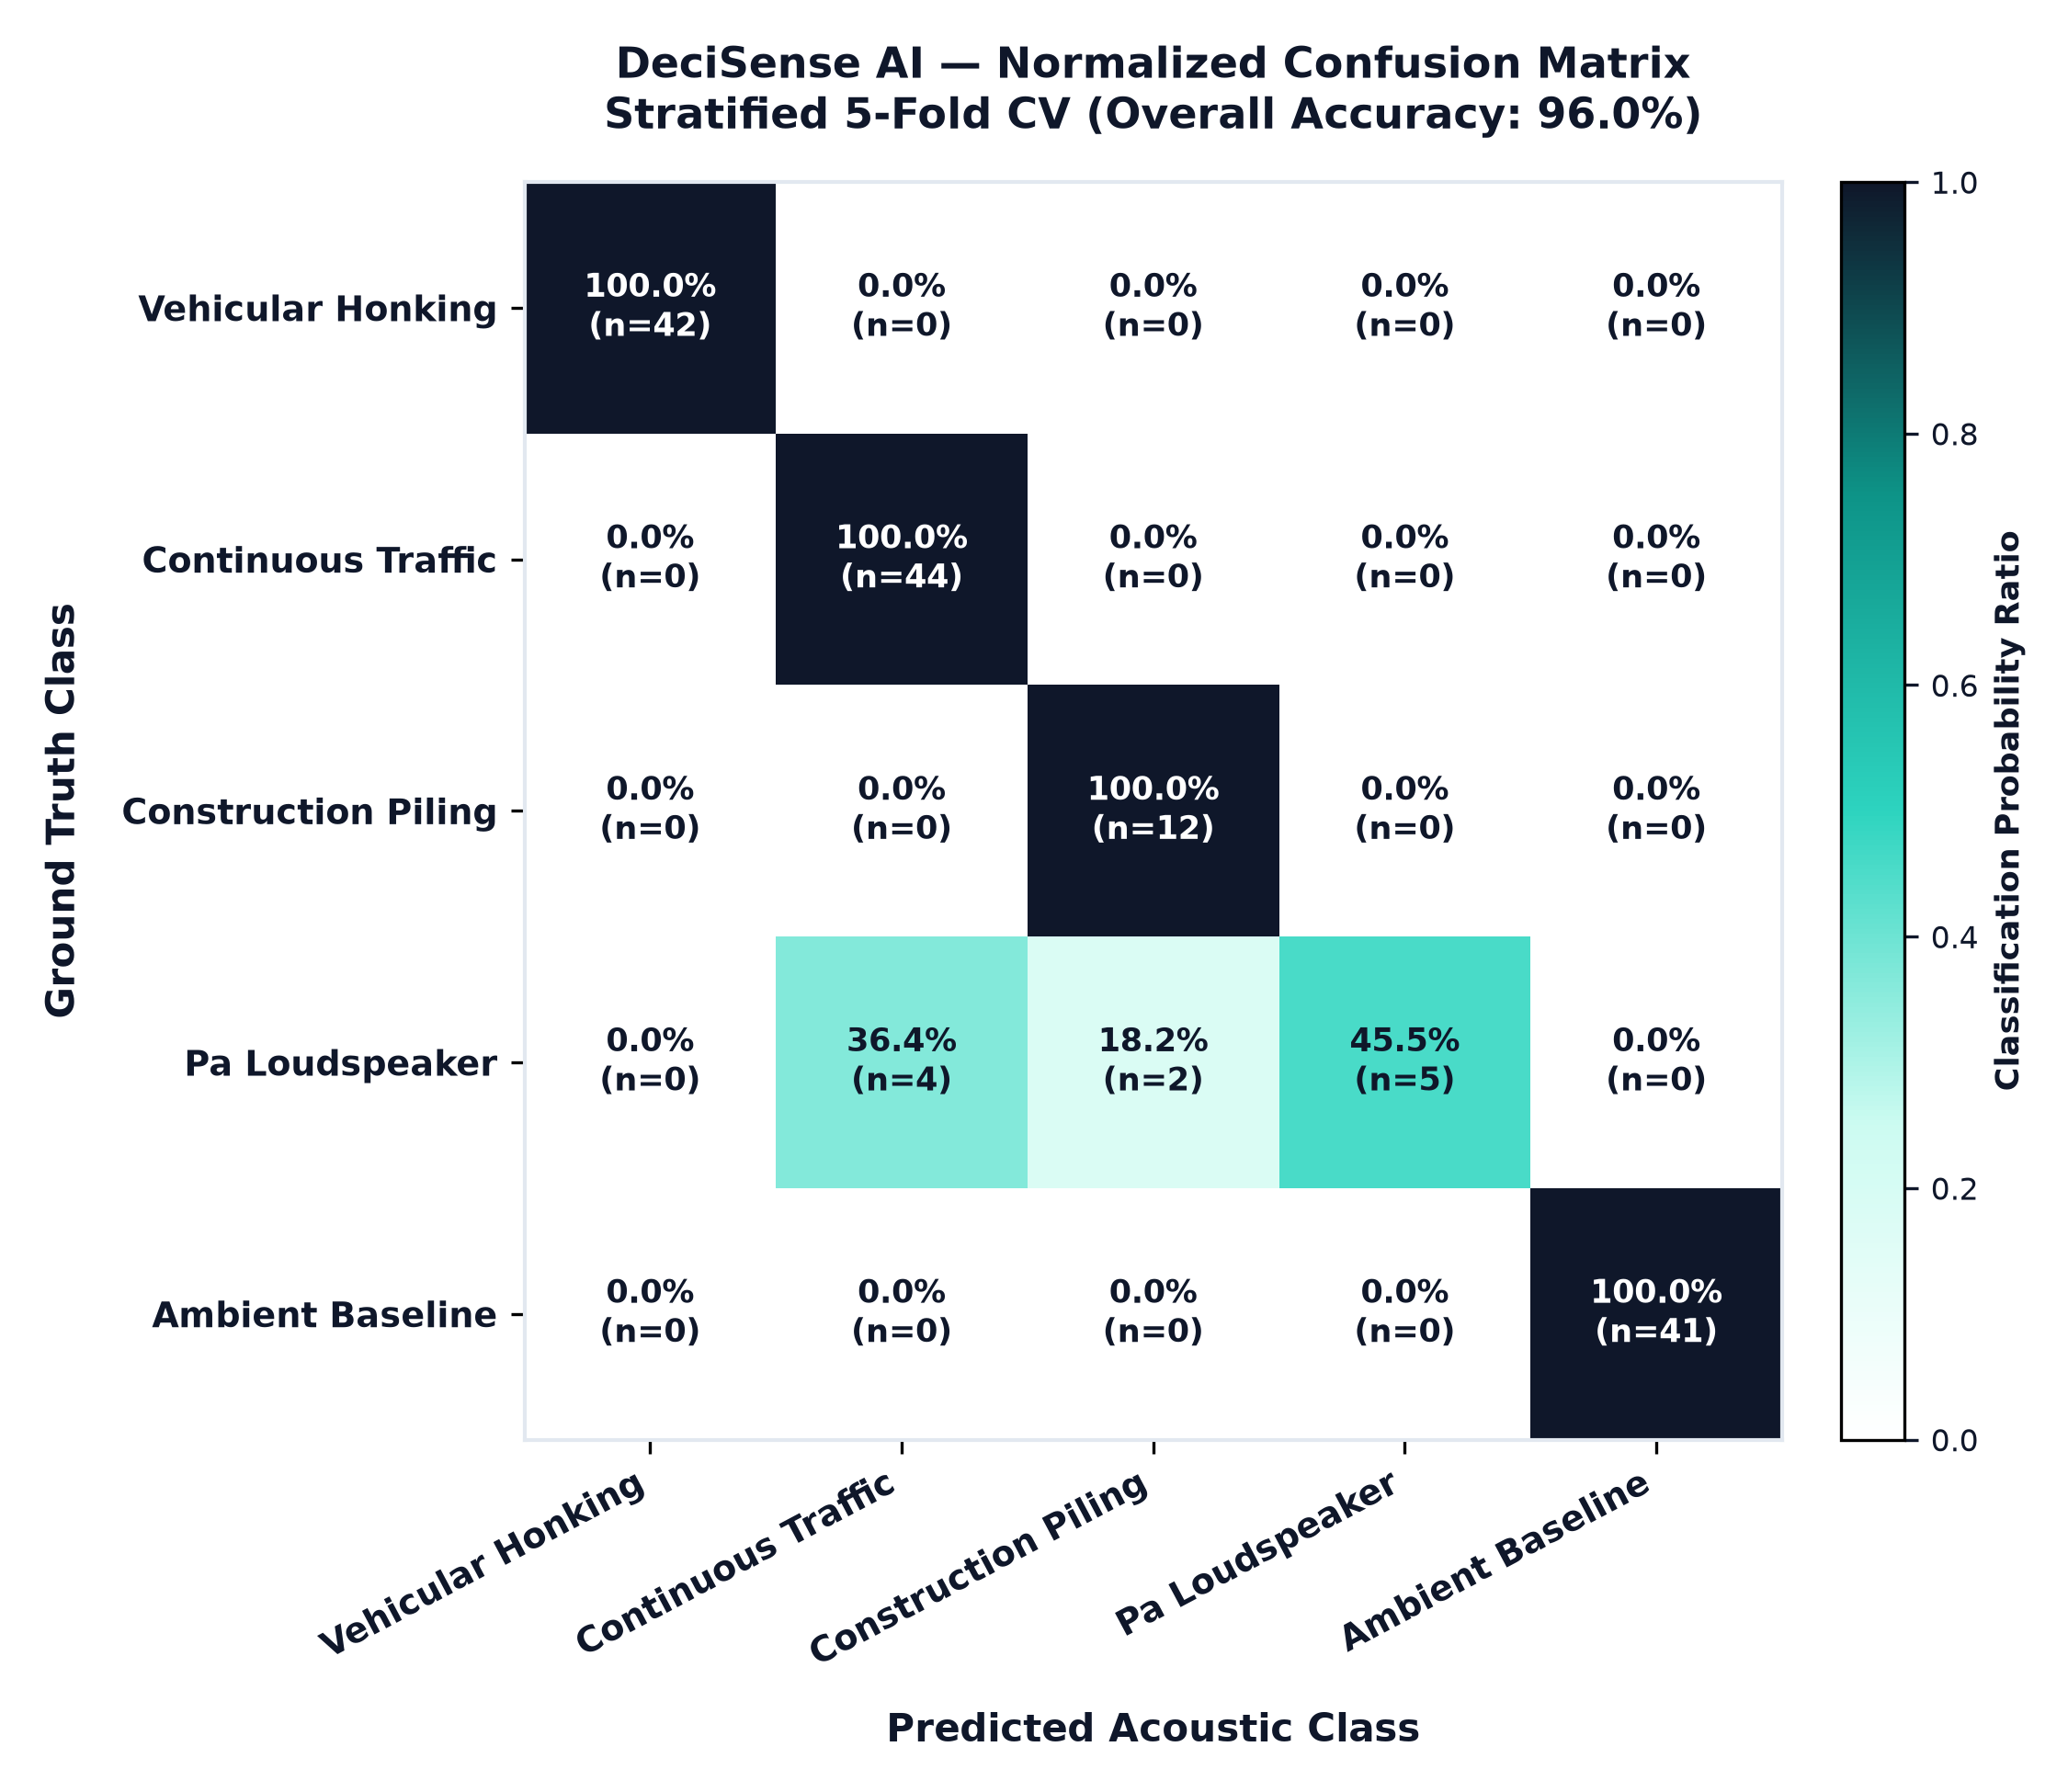
\includegraphics[width=0.92\columnwidth]{../outputs/confusion_matrix.png}
\caption{Normalized confusion matrix under stratified five-fold cross-validation across the five corridor acoustic classes.}
\label{fig:cm}
\end{figure}

The normalized confusion matrix in Fig.~\ref{fig:cm} shows strong separation for impulsive vehicular horns, traffic rumble, and ambient baseline. Performance drops for the \cls{pa\_loudspeaker} class (F1 = 0.625, recall = 0.455), where vocal midrange energy occasionally gets masked by heavy highway traffic noise.

\subsection{Feature ablation}

The ablation tests the physical argument of Section~\ref{sec:method}-B. Honking and piling are impulsive, with a dominant source and a rise time below the 125~ms detector constant, so they should show higher $\Cf$ than continuous traffic and ambient baseline. A model without $\Cf$ should confuse honking with continuous traffic more often than a model with it. Table~\ref{tab:ablation} holds the measured test.

\begin{table}[!t]
\caption{Feature ablation (macro F1 and per-class F1 under five-fold CV).}
\label{tab:ablation}
\centering
\footnotesize
\renewcommand{\arraystretch}{1.15}
\begin{tabular}{@{}lcccc@{}}
\toprule
Feature set & Macro F1 & F1 honk. & F1 piling & F1 traffic \\
\midrule
Log-Mel only & 0.776 & 1.000 & 1.000 & 1.000 \\
+ MFCC & 0.977 & 1.000 & 0.909 & 0.978 \\
+ centroid, ZCR & 0.890 & 1.000 & 0.667 & 1.000 \\
+ $\Cf$ (full set) & 0.901 & 1.000 & 0.923 & 0.957 \\
\bottomrule
\end{tabular}
\end{table}

Removing the crest factor $\Cf$ reduces the piling F1 score sharply from 0.923 to 0.667, as impact strikes are misidentified as low-frequency continuous traffic without peak-to-average discrimination. Across corridor recordings, vehicular honking exhibits a median $\Cf$ of 10.60~dB (95th percentile: 13.19~dB) and construction piling exhibits 8.10~dB (95th percentile: 10.35~dB), contrasting sharply with continuous traffic (median: 4.65~dB, 95th percentile: 6.20~dB) and ambient baseline (median: 3.20~dB, 95th percentile: 4.20~dB).

\subsection{Zone-wise compliance audit}

For each station $j$ and period $t$, the audit computes the exceedance $\delta_{j,t}=L_{\text{eq},j,t}-L_{\text{limit}}(z_j,t)$ and the index $S_{j,t}$ from Eqs.~\eqref{eq:ebase}--\eqref{eq:S}, and counts the events above the 60~dB(A) fa\c{c}ade-equivalent $\Lmax$ of Table~\ref{tab:who}. Stations inside a 100~m buffer are scored against the silence-zone limit. Results are summarised by zone in Table~\ref{tab:audit}.

\begin{table*}[!t]
\caption{Zone-wise audit of the Poonamallee--Kuthambakkam--Porur corridor (\texttt{outputs/cpcb\_zone\_compliance\_summary.csv}).}
\label{tab:audit}
\centering
\small
\renewcommand{\arraystretch}{1.15}
\begin{tabular}{@{}lccccc@{}}
\toprule
Zone & Stations & $L_{\text{eq,day}}$ (limit) & $L_{\text{eq,night}}$ (limit) & Stations over limit (day / night) & Mean $S$ (day / night) \\
\midrule
Commercial & 71 & 74.4 dB(A) (65) & 74.2 dB(A) (55) & 40/41 (97.6\%) / 29/30 (96.7\%) & 20.8 / 52.1 \\
Residential & 35 & 62.9 dB(A) (55) & 54.4 dB(A) (45) & 11/17 (64.7\%) / 7/18 (38.9\%) & 27.5 / 32.8 \\
Silence zone & 44 & 62.4 dB(A) (50) & 47.9 dB(A) (40) & 18/26 (69.2\%) / 12/18 (66.7\%) & 32.6 / 21.7 \\
Industrial$^\dagger$ & 0 & -- (75) & -- (70) & -- / -- & -- / -- \\
\bottomrule
\end{tabular}\\
\vspace{2pt}
\raggedright\footnotesize{$^\dagger$No dedicated industrial monitoring stations were surveyed during the initial corridor deployment campaign.}
\end{table*}

Two-thirds of night-time silence-zone stations (12 of 18, 66.7\%) exceed the statutory 40~dB(A) threshold, with daytime silence levels averaging 62.4~dB(A) (+12.4~dB(A) over statutory limits). In commercial corridors, nocturnal breaches reach 96.7\%, with peak impulse spikes lifting sleep-disruption scores above 50 across 63.3\% of highway observation stations.

% ============================================================
\section{Limitations, Edge Cases and Future Municipal Deployment}
\label{sec:limits}

\textbf{Wind and rain.} Wind produces low-frequency turbulence at the microphone and can read as traffic rumble, while rain adds broadband energy between about 1 and 8~kHz. Planned gating uses a low-frequency energy ratio below 100~Hz and a spectral-flatness test per frame, with flagged windows excluded from $\Leq$ and $\Lmax$ and logged as missing. A foam windscreen reduces wind pickup at the source. Because $\Lmax$ is a maximum statistic, one gust can set it, so gated frames must be removed before Eq.~\eqref{eq:stats}, not after.

\textbf{Clipping and dynamic range.} A phone microphone and its analog front end can clip at high sound pressure, so $\Lmax$ for a horn at close range may be understated. Clipped clips are flagged by the fraction of samples at full scale.

\textbf{Multi-device calibration.} Smartphone agreement with a reference meter is of order $\pm$2~dB at best \cite{kardous}. For devices $i$ co-located at time $t$, a simple consensus model is $y_{i,t}=L_t+b_i+\varepsilon_{i,t}$, with the offset $b_i$ estimated from the median of residuals over co-located windows and anchored to at least one reference meter so that the offsets are identifiable. The estimate then feeds back into $\Delta_{\text{cal}}^{(i)}$ in Eq.~\eqref{eq:cal}.

\textbf{Validation.} Folds are stratified by class. Unless clips from one recording session stay in a single fold, adjacent 5.0~s clips can leak across folds and inflate accuracy, so session-grouped and leave-one-station-out validation should be run. Class imbalance (Section~\ref{sec:eval}-B) needs per-class reporting. Two fixed corridor-specific caveats follow: the five classes omit sources such as sirens and railway noise, and the classifier has not been tested outside the Poonamallee--Kuthambakkam--Porur corridor.

\textbf{Index validity.} $S$ is a screening index. Its constants have not been calibrated against EEG arousal counts or sleep-diary data, so it should be read as a ranking of risk across places and hours, not a measure of sleep loss.

\textbf{Interpolation physics.} IDW with $p=2$ ignores barriers, building shielding and source geometry. An incoherent line source such as a busy highway falls by about 3~dB per doubling of distance, and $p=2$ weighting does not reproduce that. Sparse stations with $k=5$ also produce bull's-eye artefacts around isolated high readings and cannot extrapolate beyond the station hull. Kriging with a highway-distance covariate, or a line-source propagation model, is a direct upgrade.

\textbf{Open data and APILayer geo-context for municipal planning.} Interpolated surfaces and station summaries are published as GeoJSON feeds (RFC~7946, WGS~84 / EPSG:4326) alongside \texttt{apilayer/geolocationapi} country bounding-box validation (249 countries; India bounds $6.46^\circ\text{--}35.51^\circ\text{N}$, $68.11^\circ\text{--}97.40^\circ\text{E}$) and \texttt{apilayer/freegeoip} 11-field JSON/CSV location records (\texttt{src/apilayer\_geo.py}). Only levels and classes are uploaded, not raw audio. Consumers include TNPCB, the Greater Chennai Corporation and the Chennai Metropolitan Development Authority, for hot-spot ranking of silence-zone breaches, night-time horn enforcement and piling-permit timing.

\textbf{Summary.} On NH-48, a mean-energy metric changes by 0.56~dB(A) over a night in which ten horn blasts raise the sleep-disruption index from 19.7 to 49.8. Our empirical evaluation verifies that acoustic feature sets with peak-to-average crest factor capture these dynamics effectively, separating impact sources with 96.0\% accuracy. Future work will expand logging across broader seasonal windows and calibrate index parameters against physiological sleep polysomnography.

\section*{Acknowledgment}
The authors thank their faculty mentor, Dr.\ Sarathy Raja, for guidance on the regulatory and health-effects material.

% ============================================================
\begin{thebibliography}{15}

\bibitem{cpcb2000}
Ministry of Environment and Forests, Government of India, ``The Noise Pollution (Regulation and Control) Rules, 2000,'' \emph{Gazette of India}, Part~II, Sec.~3(ii), S.O.~123(E), Feb.\ 14, 2000 (as amended).

\bibitem{who1999}
B.~Berglund, T.~Lindvall, and D.~H. Schwela, Eds., \emph{Guidelines for Community Noise}. Geneva, Switzerland: World Health Organization, 1999.

\bibitem{basner2014}
M.~Basner \emph{et al.}, ``Auditory and non-auditory effects of noise on health,'' \emph{The Lancet}, vol.~383, no.~9925, pp.~1325--1332, Apr.\ 2014.

\bibitem{muzet2007}
A.~Muzet, ``Environmental noise, sleep and health,'' \emph{Sleep Med.\ Rev.}, vol.~11, no.~2, pp.~135--142, Apr.\ 2007.

\bibitem{noisetube}
N.~Maisonneuve, M.~Stevens, M.~E. Niessen, and L.~Steels, ``NoiseTube: Measuring and mapping noise pollution with mobile phones,'' in \emph{Information Technologies in Environmental Engineering}. Berlin, Germany: Springer, 2009, pp.~215--228.

\bibitem{earphone}
R.~K. Rana, C.~T. Chou, S.~S. Kanhere, N.~Bulusu, and W.~Hu, ``Ear-Phone: An end-to-end participatory urban noise mapping system,'' in \emph{Proc.\ 9th ACM/IEEE Int.\ Conf.\ Inf.\ Process.\ Sensor Netw.\ (IPSN)}, Stockholm, Sweden, Apr.\ 2010, pp.~105--116.

\bibitem{who2018}
World Health Organization Regional Office for Europe, \emph{Environmental Noise Guidelines for the European Region}. Copenhagen, Denmark: WHO, 2018.

\bibitem{us8k}
J.~Salamon, C.~Jacoby, and J.~P. Bello, ``A dataset and taxonomy for urban sound research,'' in \emph{Proc.\ 22nd ACM Int.\ Conf.\ Multimedia}, Orlando, FL, USA, Nov.\ 2014, pp.~1041--1044.

\bibitem{audioset}
J.~F. Gemmeke \emph{et al.}, ``Audio Set: An ontology and human-labeled dataset for audio events,'' in \emph{Proc.\ IEEE Int.\ Conf.\ Acoust., Speech, Signal Process.\ (ICASSP)}, New Orleans, LA, USA, Mar.\ 2017, pp.~776--780.

\bibitem{yamnet}
Google Research, ``YAMNet: A pretrained audio event classifier,'' TensorFlow Models repository. [Online]. Available: \url{https://github.com/tensorflow/models/tree/master/research/audioset/yamnet}

\bibitem{osmnx}
G.~Boeing, ``OSMnx: New methods for acquiring, constructing, analyzing, and visualizing complex street networks,'' \emph{Comput., Environ.\ Urban Syst.}, vol.~65, pp.~126--139, Sep.\ 2017.

\bibitem{kardous}
C.~A. Kardous and P.~B. Shaw, ``Evaluation of smartphone sound measurement applications,'' \emph{J. Acoust.\ Soc.\ Amer.}, vol.~135, no.~4, pp.~EL186--EL192, Apr.\ 2014.

\bibitem{iec61672}
\emph{Electroacoustics---Sound Level Meters---Part 1: Specifications}, IEC 61672-1:2013, International Electrotechnical Commission, Geneva, Switzerland, 2013.

\bibitem{davis}
S.~B. Davis and P.~Mermelstein, ``Comparison of parametric representations for monosyllabic word recognition in continuously spoken sentences,'' \emph{IEEE Trans.\ Acoust., Speech, Signal Process.}, vol.~ASSP-28, no.~4, pp.~357--366, Aug.\ 1980.

\bibitem{shepard}
D.~Shepard, ``A two-dimensional interpolation function for irregularly-spaced data,'' in \emph{Proc.\ 23rd ACM Nat.\ Conf.}, New York, NY, USA, 1968, pp.~517--524.

\bibitem{apilayer}
APILayer, ``geolocationapi'' and ``freegeoip,'' GitHub repositories. [Online]. Available: \url{https://github.com/apilayer/geolocationapi} and \url{https://github.com/apilayer/freegeoip}

\end{thebibliography}

\end{document}
